\section{Gleisplan}
\label{sec:map}

Dieses Kapitel stellt den aktuellen Gleisplan vor, geht aber auch auf seine historische Entwicklung ein.
Der Fokus liegt darauf, diese Entwicklung anhand der Entscheidungshintergr\"unde zu dokumentieren.
Es wird deshalb auch auf verfolgte Betriebsszenarien sowie den zugeh\"origen Dioramabau eingegangen.
Diese beiden Aspekte werden aber nachfolgend noch in unabh\"angigen Kapitel vertieft.

Da das Thema von Granitz in einer relativ flachen, Brandenburger Landschaft versiedelt ist, gibt es wenige echte Tunnels.
Zur Planung des Gleisgrundrisses wurde daher weitestgehend die Freeware \textit{Trackplanner} \cite{W\"ac07} verwendet.
Bei einigen der nachfolgenden Abbildungen handelt es sich um exportierte, i.d.R. nachbearbeitete Bilder aus der Software.
Der digitale Appendix enth\"alt zudem die Gleisplandateien im Trackplanner-typischen Format \textit{.glp}.

Nachfolgend wird zuerst die Historie des Gleisplans abgehandelt (Sec.~\ref{sec:map_basicHistory}-\ref{sec:map_History}).
Die jeweils aktuelle Ausbaustufe und der Gleisplan f\"ur die projektierte Endausbaustufe folgen in den anderen Unterkapiteln (Sec.~\ref{sec:map_date}-\ref{sec:map_final_projected}).

\subsection{Grunds\"atzliche Planungsgeschichte}
\label{sec:map_basicHistory}

Der Plan sah von Anfang an eine zweigleisige Hauptstrecke mit mindestens einer eingleisigen Nebenstrecken vor.
Es sollte dabei ein gutes Gleichgewicht zwischen Betriebsm\"oglichkeiten (Spiel) und szenerischer Gestaltung gefunden werden.
Im Fokus stand zun\"achst eine einfache Realisierung unter deutlicher Inkaufnahme eines realen Betriebsgeschehens.
Das typische Oval war dementsprechend die Grundidee.
Dieser Startschuss f\"ur Granitz kann auf \hl{ca. Weihnachten 2015} datiert werden.

Anf\"anglich war auch noch nicht klar, wann bzw. ob \"uberhaupt eine Umsetzung der Anlage ausgef\"uhrt werden k\"onnte.
Der Hauptgrund war wie so \"ublich der Platzmangel in der eigenen Wohnung, weniger der Zeitaspekt.
Im Gegenteil war letzterer absolut nachrangig, da ohnehin ein neues Hobby gesucht wurde, in dem Computer mit Hardwaresteuerung und einem vorzeigbaren Output w\"unschenswerte Bestandteile waren.

Die Arbeiten am Gleisplan wurden jeweils um Weihnachten 2018 und 2019 wiederaufgenommen.
Im Januar 2020 fiel dann auch der Entschluss, das Vorhaben tats\"achlich zu realisieren.
Durch den nach wie vor bestehenden Platzmangel wurden zun\"achst Wege gesucht, die Anlage zu segmentieren.
Ma\"sgeblich waren in diesem Zusammenhang auch Inspirationen aus Beitr\"agen, die auf der Seite \textit{moba-trickkiste.de} zusammengestellt sind.
Insbesondere ist hier der Beitrag \textit{Vom Kreisverkehr zum Betriebserlebnis} \cite{Gee17} zu nennen.
Dadurch wurde aus dem Konzept eine segmentierten Zentralplatte eine L-Form gemacht, die zu einem sp\"ateren Zeitpunkt in eine U-Form \"uberf\"uhrbar w\"are.
Die wichtigsten verarbeiteten Aspekte waren hierbei:
\begin{itemize}
	\item Raumausnutzung und An-der-Wand-F\"uhrung, was insbesondere in Plattenschenkeln von maximal 100cm Tiefe, bevorzugt weniger resultierte
	\item Ann\"aherung des Gleisplans an das Punkt-zu-Punkt Konzept
\end{itemize}
Ein weiterer Aspekt, der f\"ur Granitz aber nicht wirklich umgesetzt wurde, ist die Erkenntnis, dass eingleisige Nebenstrecken offenbar wirklich einfacher und realistischer zu bauen sind.
Sehr weit in die Zukunft schauend, w\"urden Erweiterungen oder Neubauten daher sicherlich vom zweigleisigen Hauptstreckenkonzept Abstand nehmen.

Wie man sieht, kann das Lesen aus den Erfahrungssch\"atzen anderer eine wirklich gro\"se Hilfe ist.
Mir pers\"onlich dient das zum Brinstorming und nat\"urlich auch zum aus den Fehlern anderer lernen.
Gleichwohl kann man hier und dort immer stur bleiben und den eigenen Vorstellungen folgen - das schlie\"st sich nicht aus und der Spa\"s am T\"ufteln muss ja erhalten bleiben.

Was in Hinblick auf \cite{Gee17} noch peripher erw\"ahnt sein soll - kurz losgel\"ost von der Gleisplanthematik:
Das Erz\"ahlen der fiktiven Geschichte hinter der Anlage ist denke ich sehr wichtig, um sich nicht nur selbst den Fahrplan zu legen, sondern die Anlage auch f\"ur Dritte verst\"andlich zu machen.
Aus diesem Grund erstelle ich auch die Dokumentation und es war mir ein Anliegen, die Stadt Granitz in Sec.~\ref{sec:storyOfGranitz} vorzustellen.
Das erkl\"art dann auch schon in weiten Teilen den Hintergrund zum Gleisplan, Betrieb, Szenerie etc.


\subsection{Entwicklungsstadien}
\label{sec:map_history}

\subsubsection{Das Oval}
Der etwaige Erstentwurf aus dem Jahr \hl{2015} sowie die Wiederbelebung nach Weihnachten 2018 sind in Fig.~\ref{img:state0-1_granitz_modules_details} dargestellt.
Meiner Erinnerung nach sind die einzigen Unterschiede das Fehlen der kompletten Schattenbahnhofsebene sowie des linksoben angeflanschten Nebenszenarios (Minibahnhof) - dies war im Erstentwurf nicht enthalten.
Stattdessen sollte linksoben eine \"Uberf\"uhrungsm\"oglichkeit zur Anlage meines Vaters freigehalten werden.
Die \"Uberf\"uhrung rechtsoben war jederzeit untergeordnet, da hier keine konkreten Pl\"ane vorlagen.
Eine Vereinigung mit einer Anlage meines Bruders war noch am ehesten in meiner Vorstellung.

Die Abbildung enth\"alt bereits eine Segmentierung, um die gut $2~m \cdot 3~m$ gro\"se Anlage irgendwo verstauen zu k\"onnen.
Der mittlere Segmentriegel wurde in die beiden \"au\"seren Bahntrassensegmente und die zentralen Dioramasegmente unterteilt, um letztere v\"ollig unabh\"angig entwickeln und bei Bedarf sogar ersetzen zu k\"onnen.

Das angeflanschte Segment mit dem Minibahnhof wurde als kleines, aber feines Diorama Highlight geplant.
Hier sollte ein sehr, sehr niedrig frequentierter Haltepunkt eingef\"ugt werden, der bei Ausfl\"uglern sehr beliebt ist.
Der Halt sollte auf einer Erhebung sein mit Ausblick auf den n\"ordlichen, etwa $10~cm$ tiefer gelegenen Anlagenriegel.
Noch vor der Kurve der Hauptstrecke sollte eine beschauliche Wiese mit einem kleinen Teich angelegt werden.
Die Kurve der Hauptstrecke wurde relativ bald unter das Terrain verlegt, um die Landschaft hier noch etwas weiter zu ziehen.
\begin{itemize}
	\item Das Diorama ist auch noch aktuell in Planung und wird als Bahnhof \textbf{Sch\"onblick} gelistet.
\end{itemize}

Der Regionalzug- und Bummelzughalt, oben zentral eingezeichnet, sollte als Endpunkt der hier sehr kurzen Nebenstrecke und optionaler Regionalzuhalt dienen.
Hier sollte ein durch einen Wald abgetrennter, ggf. eingemeindeter Ortsteil von Granitz angedeutet sein, urspr\"unglich als \textbf{Granitzer Heide} gelistet.
Westlich von der Bahnhofsausfahrt ergibt sich neben der Gleisf\"uhrung nach Sch\"onblick au\"serdem eine Abfahrt in die Schattenbahnhofsebene, potenziell f\"ur den G\"utervekehr.
\begin{itemize}
	\item Der Regionalzughalt ist in der aktuellen Planung als Bahnhof \textbf{Granitz-Walddorf} umgewidmet.
	\item Dioramatechnisch sehen alle fortgeschrittenen Planungen eine Trennung dieses Bahnhofs von der benachbarten Gleisaufgabelung vor.
\end{itemize}

Die zentralen Panoramasegmente sowie das Segment der Stadt Granitz selbst sind aus Fig.~\ref{img:state0-1_granitz_modules_details} heraus selbsterkl\"arend.
Der Schattenbahnhof hat allein die Funktion von Abstellgleisen und einer gro\"sen Wendeschleife, die zwischen Nordwest und S\"udost befahren werden kann.
Allein ein Merkmal soll hier explizit aufgef\"uhrt werden, das f\"ur alle Entwurfsphasen mandatorisch war und ist:
\begin{itemize}
	\item Bahnsteige m\"ussen eine Kapazit\"at von mindestens f\"unf (Fernverkehr) bzw. vier  (Regionalverkehr) Personenwagen aufweisen.
	Dies gibt somit die Bahnsteigl\"angen in Granitz sowie am Regionalhalt vor.
	\item Eine Kapazit\"at von sechs Personenwagen in Granitz ist dar\"uber hinaus ausdr\"ucklich angestrebt.
\end{itemize}

Modelleisenbahnanlagenbau kann viel Zeit in Anspruch nehmen.
F\"ur mich war und ist es wichtig, bald schon mal einen Zug fahren lassen zu k\"onnen.
Zusammen mit den bereits angedeuteten Problemen bzgl. Platzmangels in der Wohnung wurde schon sehr fr\"uh die Modularisierung in Segmente auf den Plan gesetzt.
Insbesondere 2018 erschien es als absolut unrealistisch, eine Plattentiefe von $2m$ in der Wohnung zu realisieren.
Als Kombil\"osung beide Aspekte betreffend wurde die komplette Entnahme des mittleren Segmentriegels als Option geplant, s. Fig.~\ref{img:state0-1_granitz_modules_compressed}.

Dies erfordert f\"ur eine Anpassung der (urspr\"unglichen) finalen Anlage gem\"a\"s Fig.~\ref{img:state0-1_granitz_modules_details} wenig \"Anderungen an der Gleisf\"uhrung:
\begin{enumerate}
	\item Die Nebenstrecke braucht eine alternative, flachere Zuf\"uhrung zum Regionalhalt.
	Dies kann auch bei einem m\"oglichen Hin- und Herwechseln zwischen der komprimierten und Vollvariante bestehen bleiben, indem \"uber eine zus\"atzliche, am Westausgang vom Bummelzughalt einzubauende Weiche (hier nicht abgebildet) jeweils das nicht genutzt Gleis als Totgleis definiert wird.
	\item Der westliche Schleifenschluss in der Schattenbahnhofsebene erfordert eine geringf\"ugige Anpassung.
\end{enumerate}
Es sei darauf verwiesen, dass der mittlere Segmentriegel mit eine Tiefe von $55.5~cm$ bemessen wurde, dementsprechend auf Standardl\"angen vom verwendeten Gleismaterial ausgelegt wurde.

Als zus\"atzliche Information enth\"alt Fig.~\ref{img:state0-1_granitz_modules_compressed} verschiedene Baulose f\"ur den Bastler.
Diese waren sowohl in zeitlich und gestalterisch sinnvolle Abschnitte unterteilt als auch in Budgetierungsabschnitte, um den geringen Gleisbestand aus der Kinderanlage haushaltspolitisch vertr\"aglich zu erweitern.

\begin{figure}[h]
\centering
	\begin{subfigure}[b]{1.0\textwidth}
    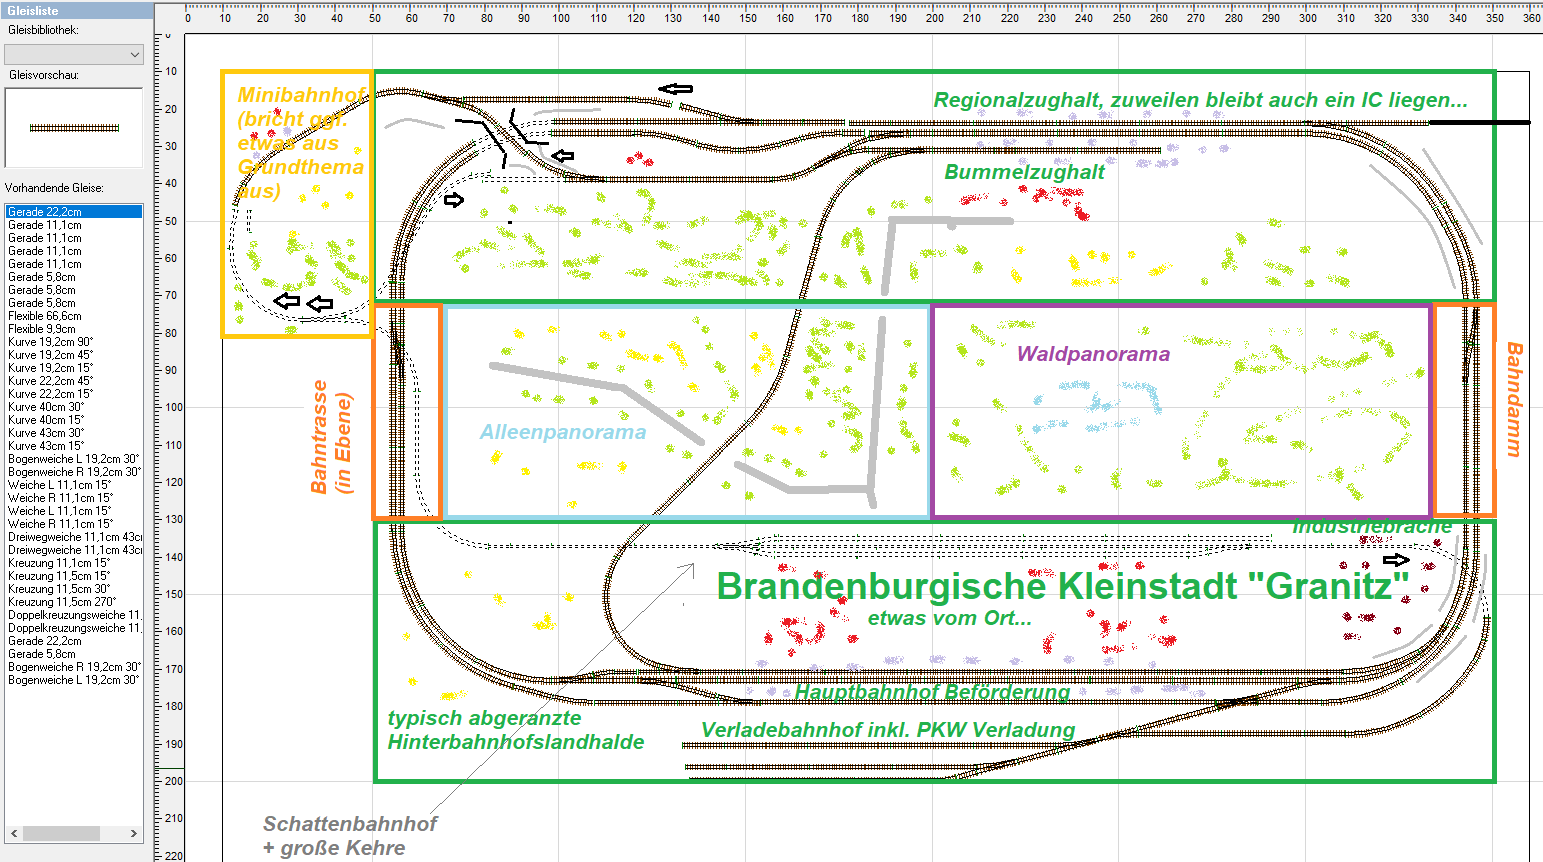
\includegraphics[width=1.0\textwidth]{img/map_evolution/state0-1_granitz_modules_details.png}
   \caption{Urspr\"ungliche Planung f\"ur Vollausbau}
    \label{img:state0-1_granitz_modules_details}
    \end{subfigure}
	\begin{subfigure}[b]{1.0\textwidth}
    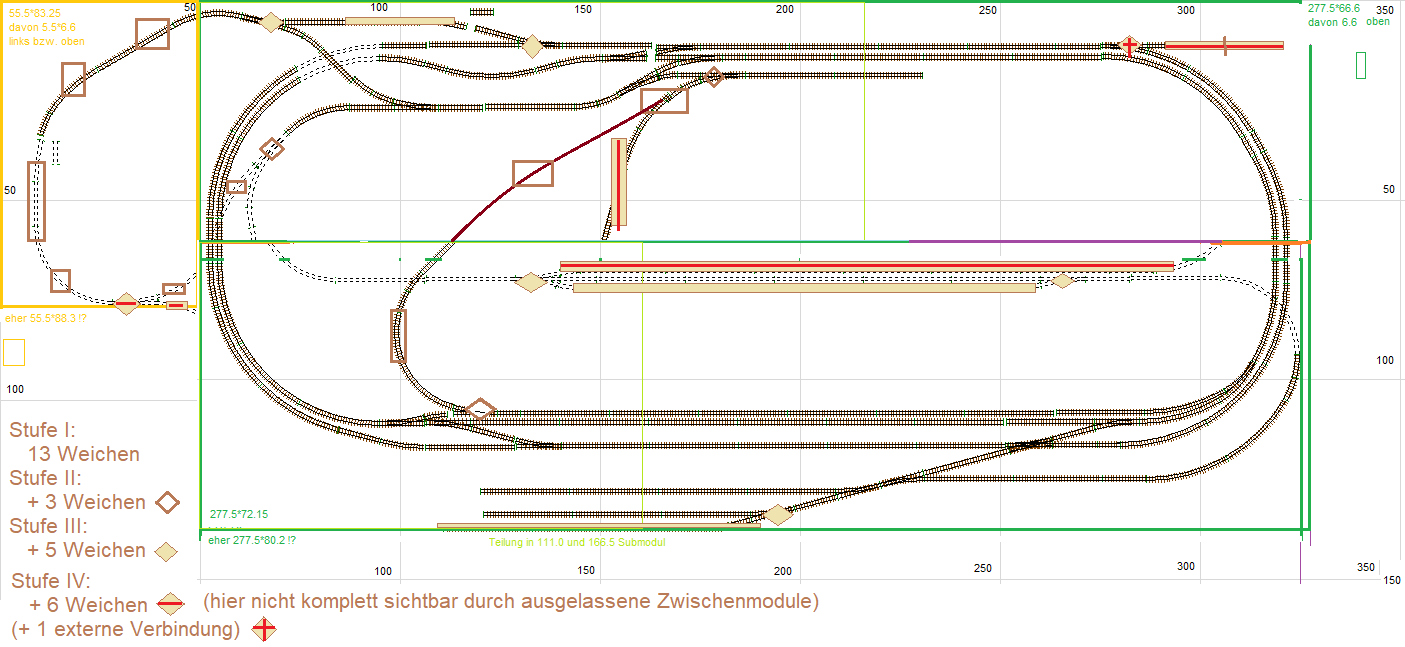
\includegraphics[width=1.0\textwidth]{img/map_evolution/state0-1_granitz_modules_compressed.png}
   \caption{Komprimierte Anlage f\"ur fr\"uhe Ausbaustadien}
    \label{img:state0-1_granitz_modules_compressed}
    \end{subfigure}
	\label{img:state0-1_granitz}
	\caption{Erste Entwurfsserie, ausgef\"uhrt als segmentierte Rechteckanlage}
\end{figure}

Letztendlich entsprechen diese Erstentw\"urfe dem klassischen Oval mit etwas Nebenstreckenfirlefans.
Das war dem Autor fr\"uh bewusst aber auch okay so.
Es ging darum, mal einen Zug fahren zu lassen, etwas \"uber die Nebenstrecken und mit dem Schattenbahnhof zu variieren und sich vor allem an den beiden Panoramaplatten gestalterisch auszutoben.
Siehe hierzu auch die in der Einleitung beschriebene Geisterung f\"ur Brandenburg und das ganze drum herum.
Die Fahrstrecke zwischen Granitz und dem Regionalhalt war mit ca. $3m$ (\"uber Granitz-West) bzw. ca. $2m$ (\"uber Granitz-Ost) auch annehmbar.


\subsubsection{Ann\"aherung an den Hundeknochen \"uber die Acht}



\begin{figure}[h]
\centering
  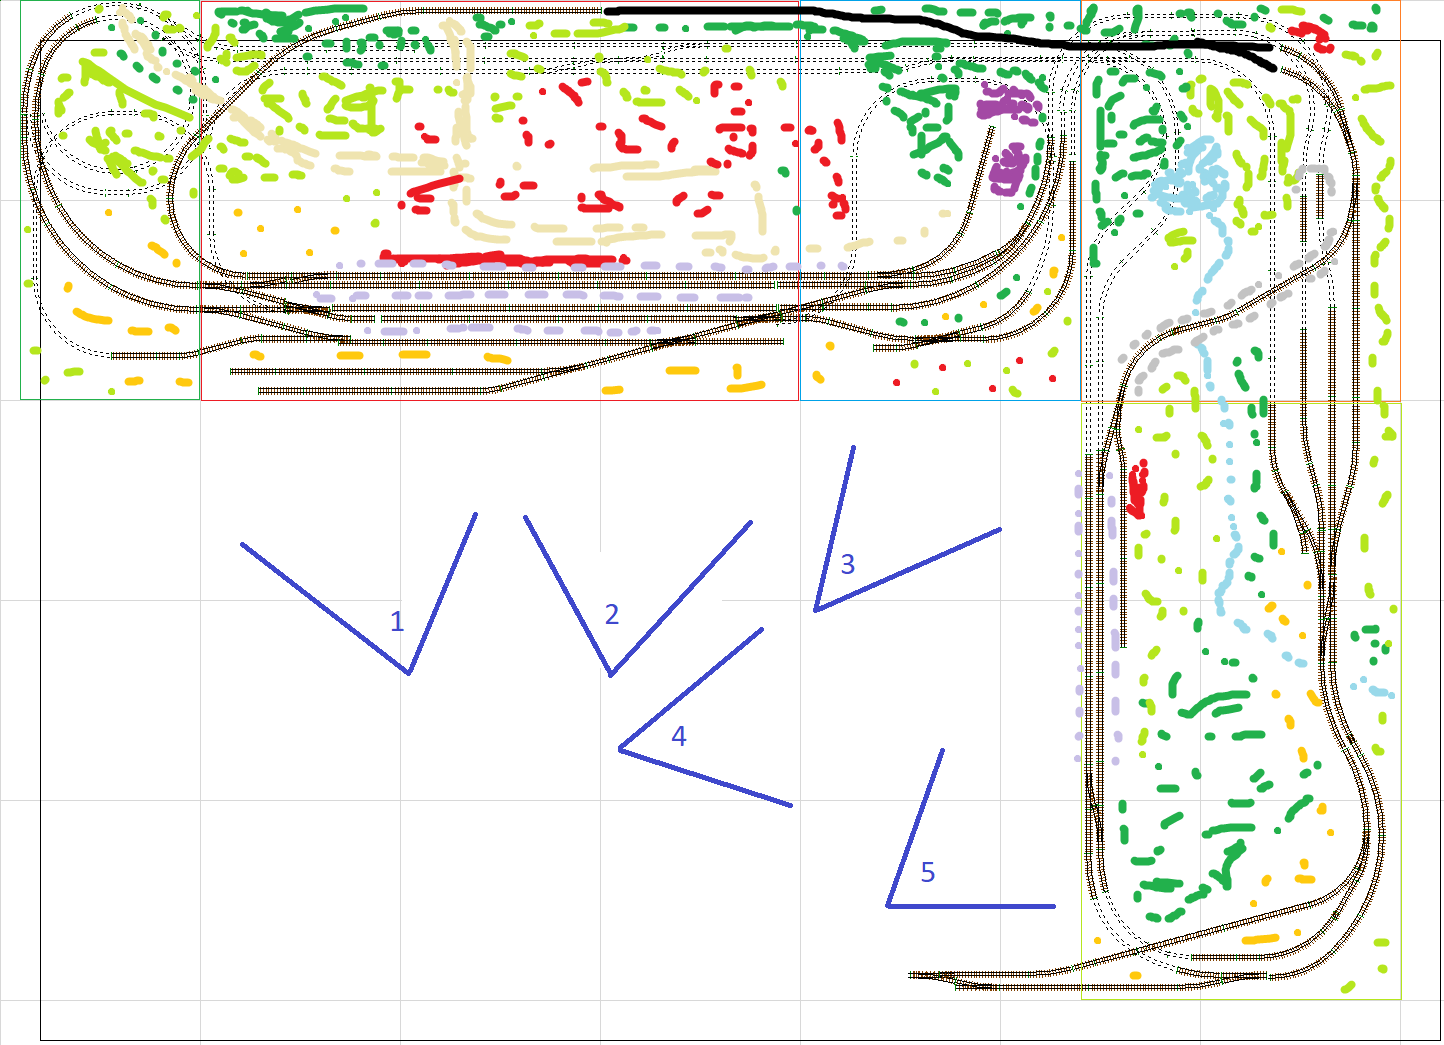
\includegraphics[width=1.0\textwidth]{img/map_evolution/state2_granitz_modules_details.png}
	\label{img:state2_granitz_modules_details}
	\caption{Erste Entwurfsserie, ausgef\"uhrt als segmentierte Rechteckanlage}
\end{figure}





\subsubsection{Ann\"aherung an das Eigentliche Punkt zu Punkt Konzept}


\begin{figure}[h]
\centering
  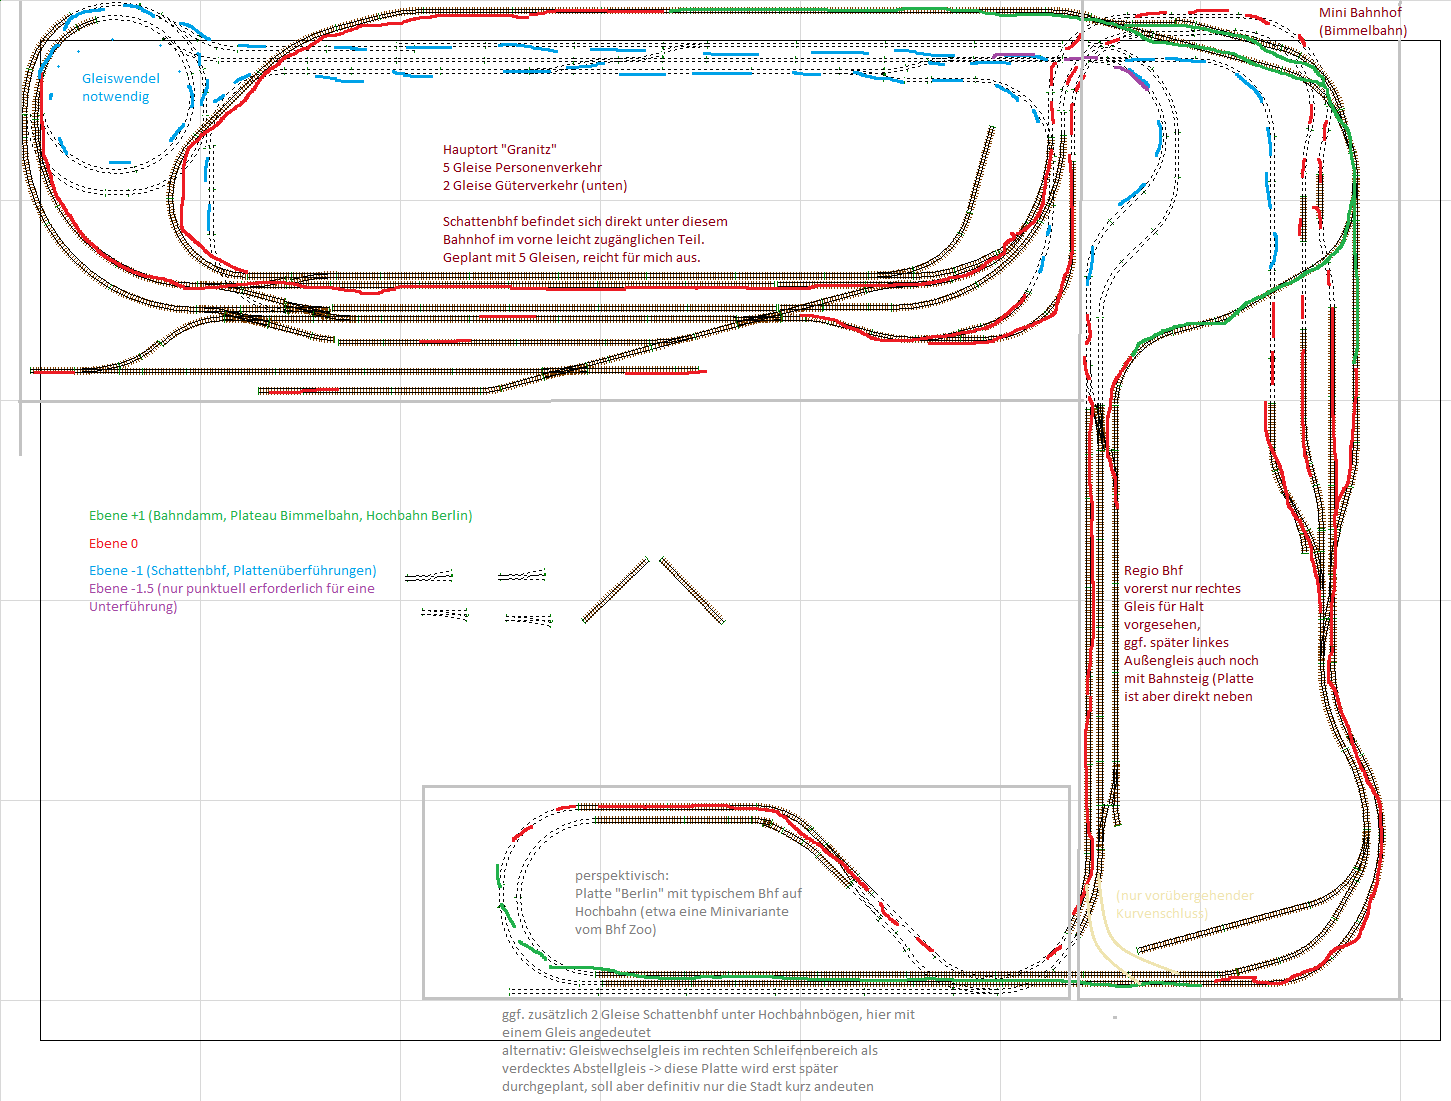
\includegraphics[width=1.0\textwidth]{img/map_evolution/state3_granitz_modules.png}
	\label{img:state3_granitz_modules}
	\caption{Erste Entwurfsserie, ausgef\"uhrt als segmentierte Rechteckanlage}
\end{figure}


\subsection{Aktueller Gleisplan}
\label{sec:map_date}



\subsection{Projektierter Endausbau}
\label{sec:map_final_projected}


%\begin{figure}[h]
%\centering
	%\begin{subfigure}[b]{0.49\textwidth}
    %\includegraphics[width=1.0\textwidth]{sub/concept_studies/img/carpets/benefit_maps/map_benefit_s500.png}
   %\caption{$s = 500 NM$}
    %\label{img:carpets_benefit_maps_s500}
    %\end{subfigure}
	%\begin{subfigure}[b]{0.49\textwidth}
    %\includegraphics[width=1.0\textwidth]{sub/concept_studies/img/carpets/benefit_maps/map_benefit_s1000.png}
   %\caption{$s = 1000 NM$}
    %\label{img:carpets_benefit_maps_s1000}
    %\end{subfigure}
		%\begin{subfigure}[b]{0.49\textwidth}
    %\includegraphics[width=1.0\textwidth]{sub/concept_studies/img/carpets/benefit_maps/map_benefit_s2500.png}
   %\caption{$s = 2500 NM$}
    %\label{img:carpets_benefit_maps_s2500}
    %\end{subfigure}
		%\begin{subfigure}[b]{0.49\textwidth}
    %\includegraphics[width=1.0\textwidth]{sub/concept_studies/img/carpets/benefit_maps/map_benefit_s5000.png}
   %\caption{$s = 5000 NM$}
    %\label{img:carpets_benefit_maps_s5000}
    %\end{subfigure}
	%\label{img:carpets_benefit_maps}
	%\caption{Straight map of benefits for PSN supply flow modulation}
%\end{figure}